\documentclass[11pt,letter, swedish, english
]{article}
\pdfoutput=1

\usepackage{../custom_as}
\usepackage[makeroom
]{cancel}
\usepackage{esint}
\let\oldint\int 
\renewcommand{\int}{\oldint\limits}
\graphicspath{{figures/}}

\swapcommands{\Phi}{\varPhi}
\swapcommands{\Omega}{\varOmega}
\swapcommands{\Sigma}{\varSigma}
\swapcommands{\Lambda}{\varLambda}

\swapcommands{\epsilon}{\varepsilon}


\newcommand{\enaught}{\ensuremath\varepsilon_0}

%%Drar in tabell och figurtexter
\usepackage[margin=10 pt]{caption}
%%För att lägga in 'att göra'-noteringar i texten
\usepackage{todonotes} %\todo{...}

%%För att själv bestämma marginalerna. 
\usepackage[
%            top    = 2.5cm,
%            bottom = 3cm,
%            left   = 3cm, right  = 3cm
]{geometry}

%%För att ändra hur rubrikerna ska formateras


%\renewcommand{\thefootnote}{\fnsymbol{footnote}}

%\newcommand{\Tc}{\ensuremath{T_{\text{c}}}}
\newcommand{\sign}{\ensuremath{\,\text{sign}}}

%\usepackage{tikz}


\renewcommand{\thesubsection}{\arabic{section} (\alph{subsection})}
\renewcommand{\thesubsubsection}{\arabic{section} (\alph{subsection},\,\roman{subsubsection})}


\begin{document}

%\tikzstyle{every picture}+=[remember picture]
%\tikzstyle{na} = [shape=rectangle,inner sep=0pt,text depth=0pt]



%%%%%%%%%%%%%%%%% vvv Inbyggd titelsida vvv %%%%%%%%%%%%%%%%%

\title{E\&M -- PHYS\,706 \\
Assignment 1}
\author{Andréas Sundström}
\date{\today}

\maketitle

%%%%%%%%%%%%%%%%% ^^^ Inbyggd titelsida ^^^ %%%%%%%%%%%%%%%%%

\section*{Boundary conditions}
Before we begin, I will just list the boundary conditions for the
electromagnetic field at a boundary, see Jackson (I.17)--(I.20). The
boundary conditions are
\begin{align}
&(\vb*E_1 - \vb*E_2)\cross\vu{n}_{12} = 0     \label{eq:01}\\
&(\vb*D_2 - \vb*D_1)\vdot\vu{n}_{12} = \sigma \label{eq:02}\\
&(\vb*H_1 - \vb*H_2)\cross\vu{n}_{12} = \vb*j \label{eq:03}\\
&(\vb*B_1 - \vb*B_2)\vdot\vu{n}_{12} = 0,     \label{eq:04}
\end{align}
where $\vu{n}_{12}$ is a normal to the interface pointing from region 1
to 2, $\sigma$ is the surface charge density at the interface, and
$\vu*j$ is the surface current density at the interface. These
boundary conditions will be useful in the following problems. 

\section{Three indices of refraction -- normal incidence}
\newcommand{\Ep}{{\mathcal{E}_1^+}}
\newcommand{\Epp}{{\mathcal{E}_2^+}}
\newcommand{\Eppp}{{\mathcal{E}_3^+}}
\newcommand{\Em}{{\mathcal{E}_1^-}}
\newcommand{\Emm}{{\mathcal{E}_2^-}}

In this problem we have a normally incident wave, with wavenumber
$k_0=2\pi/\lambda_0$, at an interface to a second media of finite
width $d$; after the waves has passed through the second region, it
enters a third region that is infinite. The three regions have indices
of refraction $n_1=1$, $n_2$ and $n_3$. All of this together with some 
definition of notation are shown in \figref{fig:1_geometry}.

\begin{figure}
\centering
\resizebox{.6\textwidth}{!}{\input{figures/1_geometry.pdf_t}}
\caption{Three different regions all with their own index of
  refraction. This figure also shows the notation used for the
  different fields. }
\label{fig:1_geometry}
\end{figure}

This problem will require the use of the boundary conditions
\eqref{eq:01} and \eqref{eq:03} with $\vb*j=0$. To use
these boundary conditions we must first establish expressions for the
fields:
\begin{equation}
\begin{aligned}
\vb*E_1^\pm=&\vu{x}\mathcal{E}_1^\pm\ee^{\pm\ii k_1z -\ii\omega t}\\
\vb*E_2^\pm=&\vu{x}\mathcal{E}_2^\pm\ee^{\pm\ii k_2z -\ii\omega t}\\
\vb*E_3^{+}=&\vu{x}\mathcal{E}_3^+\ee^{+\ii k_3z -\ii\omega t},
\end{aligned}
\end{equation}
where $k_i=n_ik_0=n_i2\pi/\lambda_0$. We see that since $\omega$
is the same for all, we can drop the factor $\ee^{-\i\omega t}$ in all
further calculations. 

We also note that all the fields are in the $\vu{x}$ direction, all
wavevectors are in the $\pm\vu{z}$ direction, and
$\vu{n}_{12}=\vu{z}$, so it will be sufficient to work with the
complex amplitudes and phases. With this observation we are ready to
write down the boundary conditions for each boundary. 

First the $z=0$ boundary, where \eqref{eq:01} gives
\begin{equation}
\Ep+\Em -(\Epp+\Emm) =0, 
\end{equation}
and \eqref{eq:03} gives
\begin{equation}
\frac{k_1}{\mu_1}\qty(\Ep-\Em) 
-\frac{k_2}{\mu_2}\qty(\Epp-\Emm) =0.
\end{equation}
In the last step we used the fact that 
$\vb*H = \vb*B/\mu = \vb*k\cross\vb*E/(\omega\mu)$. The different
signs between ``$+$'' and ``$-$'' amplitudes are due to the fact that
they travel in different directions. 

Similarly for the $z=d$ boundary, now we do however need to keep the
complex phases, due a to non-zero $z$ value, in mind. Nonetheless the
result is similar. From \eqref{eq:01} we get
\begin{equation}
\Epp\ee^{\ii k_2d}+\Emm\ee^{-\ii k_2d} -\Eppp\ee^{\ii k_3d} =0, 
\end{equation}
and from \eqref{eq:03} we get
\begin{equation}
\frac{k_2}{\mu_2}\qty(\Epp\ee^{\ii k_2d}-\Emm\ee^{-\ii k_2d}) 
-\frac{k_3}{\mu_3}\Eppp\ee^{\ii k_3d} =0.
\end{equation}

We now have four equations and four unknowns (given $\Ep$, the
unknowns are $\Em$, $\Epp$, $\Emm$, and $\Eppp$). Furthermore, the
equations are all linear, meaning that we can write them on matrix
form
\begin{equation}\label{eq:1_master}
\begin{bmatrix}
+1 & -1 & -1 & 0 \\
-K_1 & -K_2 & +K_2 &0\\
0& \ee^{\ii k_2d}& \ee^{-\ii k_2d}& -\ee^{\ii k_3d}\\
0& K_2\ee^{\ii k_2d}& -K_2\ee^{-\ii k_2d}& -K_3\ee^{\ii k_3d}\\
\end{bmatrix}
\begin{bmatrix}
\Em \\ \Epp \\ \Emm \\ \Eppp
\end{bmatrix}
= \Ep
\begin{bmatrix}
-1 \\ -K_1 \\ 0 \\ 0
\end{bmatrix},
\end{equation}
where $K_i:=k_i/\mu_i$. This linear system of equations is not trivial
to solve, but the methods needed are (first year linear algebra), so I
will let \textit{Mathematica} do the grunt work and solve this system
for me. 

To simplify the expressions a bit we set $\mu_1=\mu_2=\mu_3$, and also
remember that $k_i=k_0n_i$. With this in mind, we get the raw output
from Mathematica:
\begin{equation}\label{eq:1_Em}
\frac{\Em}{\Ep}=
\frac{
n_1 (n_2(1 + \ee^{2\ii dk_0n_2}) + n_3(1 - \ee^{2\ii dk_0n_2})) + 
 n_2 (n_2(-1 + \ee^{2\ii dk_0n_2}) - n_3(1 + \ee^{2\ii dk_0n_2}))
}{
n_1 (n_2(1 + \ee^{2\ii dk_0n_2}) + n_3(1 - \ee^{2\ii dk_0n_2})) + 
 n_2 (n_2(1 - \ee^{2\ii dk_0n_2}) + n_3(1 + \ee^{2\ii dk_0n_2}))
}
\end{equation}
and 
\begin{equation}\label{eq:1_Eppp}
\frac{\Eppp}{\Ep} = 
\frac{
4n_1n_2 \ee^{\ii d k_0(n_2-n_3)}
}{
n_1 (n_2(1 + \ee^{2\ii dk_0n_2}) + n_3(1 - \ee^{2\ii dk_0n_2})) + 
 n_2 (n_2(1 - \ee^{2\ii dk_0n_2}) + n_3(1 + \ee^{2\ii dk_0n_2}))
}
\end{equation}
The other two outputs, $\Epp$ and $\Emm$, will not be relevant to the
rest of the problem, so they are omitted here. 




\subsection{Reflectivity}
In this part of the problem we want to calculate the reflectivity
$R=|\Em/Ep|^2$. By studying \eqref{eq:1_Em}, we see that we can
multiply both the numerator and denominator by $\ee^{-\ii dk_0n_2}/2$ to
get
\begin{equation}
\frac{\Em}{\Ep}=
\frac{
n_1 (n_2\cos(dk_0n_2) -\ii n_3\sin(dk_0n_2)) + 
 n_2 (\ii n_2\sin(dk_0n_2) - n_3\cos(dk_0n_2))
}{
n_1 (n_2\cos(dk_0n_2) - \ii n_3\sin(dk_0n_2)) + 
 n_2 (-\ii n_2\sin(dk_0n_2) + n_3\cos(dk_0n_2))
}.
\end{equation}
If we now collect all the cosines and sines, we get
\begin{equation}
\frac{\Em}{\Ep}=\frac{
n_2(n_1-n_3)\cos(dk_0n_2) +\ii(n_2^2 -n_1n_3)\sin(dk_0n_2)
}{
n_2(n_1 +n_3)\cos(dk_0n_2) - \ii(n_2^2 +n_1n_3)\sin(dk_0n_2) 
}.
\end{equation}

And finally the reflectivity is the ration of reflected over incident
\emph{intensity}. Since both the incident and reflected wave travel in
the same media we can just write
\begin{equation}
R =\frac{I_1^-}{I_2^+}= \abs{\frac{\Em}{\Ep}}^2=
\frac{
\Big[n_2(n_1-n_3)\cos(dk_0n_2)\Big]^2 
+\Big[(n_2^2 -n_1n_3)\sin(dk_0n_2)\Big]^2
}{
\Big[n_2(n_1 +n_3)\cos(dk_0n_2)\Big]^2 
+\Big[(n_2^2 +n_1n_3)\sin(dk_0n_2)\Big]^2 
},
\end{equation}
where $k_0=2\pi/\lambda_0$.

A plot of $R$ as a function of $d/\lambda_0$ is shown in
\figref{fig:1a_R}. 


\begin{figure}
\centering
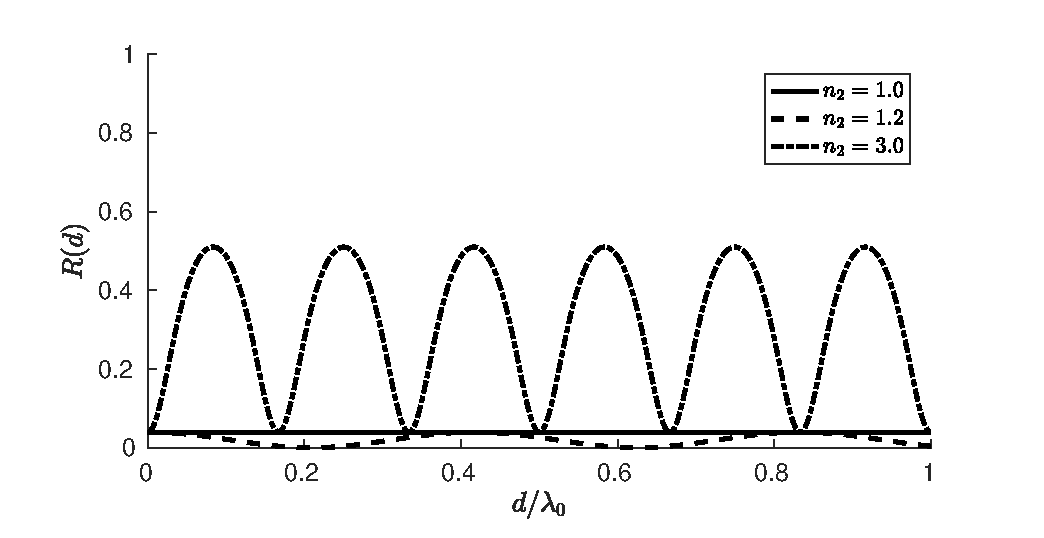
\includegraphics[width=.9\textwidth]{1a_R.eps}
\caption{The reflectivity as a function of slab thickness $d$. The
  reflectivity is for $n_1=1$, $n_3=1.5$ and $n_2=1.0, 1.2$ and 3.}
\label{fig:1a_R}
\end{figure}


\subsection{Transmitivity}
Here we start off from \eqref{eq:1_Eppp}, and do almost the same
procedure as above. But we can begin by noting that the denominator is
exactly the same in \eqref{eq:1_Eppp} as in \eqref{eq:1_Em}. So by
multiplying both the numerator and denominator by $\ee^{-\ii dk_0n_2}/2$,
we get
\begin{equation}
\begin{aligned}
\frac{\Eppp}{\Ep} =&
\frac{
4n_1n_2 \ee^{\ii d k_0(n_2-n_3)} \times \ee^{-\ii dk_0n_2}/2
}{n_2(n_1 +n_3)\cos(dk_0n_2) - \ii(n_2^2 +n_1n_3)\sin(dk_0n_2) 
}\\
=&
\frac{
2n_1n_2 \ee^{-\ii d k_0n_3} 
}{n_2(n_1 +n_3)\cos(dk_0n_2) - \ii(n_2^2 +n_1n_3)\sin(dk_0n_2) 
}.
\end{aligned}
\end{equation}

For the transmitivity $T=I_3^+/I_1^+$, it is not as straight forward
as just squaring the absolute values. Since the intensity of a wave is
given by
\begin{equation}
I = \frac{1}{2} \epsilon v \abs{E}^2 
= \frac{1}{2} n^2\frac{\epsilon_0\mu_0}{\mu} \,\frac{c}{n} \abs{E}^2 
= \frac{1}{2} \frac{n}{\mu c} \abs{E}^2. 
\end{equation}
The transmitivity should therefore be
\begin{equation}
T = \frac{I_3^+}{I_1^+} 
= \frac{\frac{n_3}{\mu c}\abs{\Eppp}^2}{\frac{n_1}{\mu c}\abs{\Ep}^2}
= \frac{n_3}{n_1}\,\abs{\frac{\Eppp}{\Ep}}^2.
\end{equation}
This gives
\begin{equation}
T =
\frac{
4n_1n_3\,n_2^2
}{
\Big[n_2(n_1 +n_3)\cos(dk_0n_2)\Big]^2 
+\Big[(n_2^2 +n_1n_3)\sin(dk_0n_2)\Big]^2 
}
\end{equation}
where $k_0=2\pi/\lambda_0$.

A plot of $T$ as a function of $d/\lambda_0$ is shown in
\figref{fig:1b_T}. 

\begin{figure}
\centering
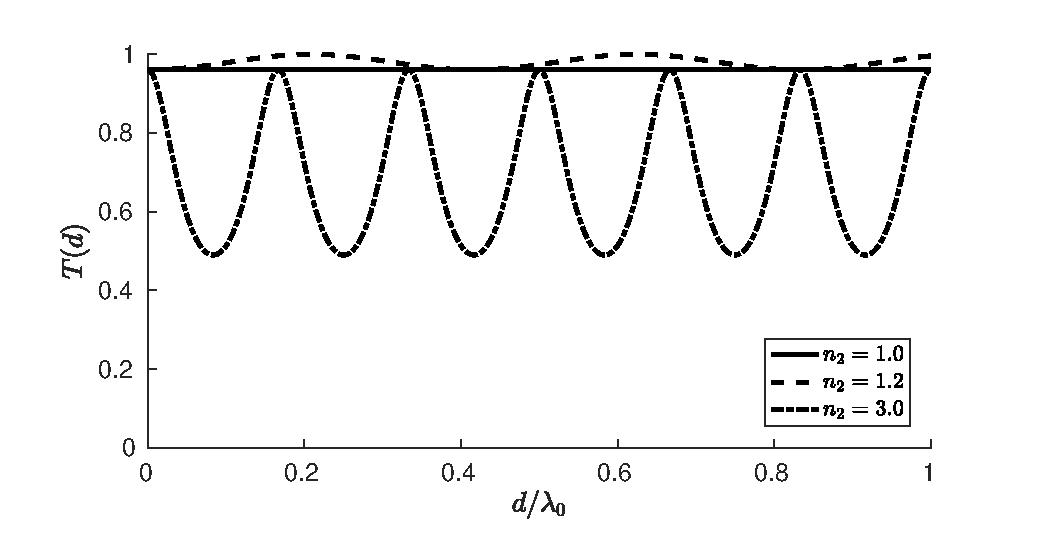
\includegraphics[width=.9\textwidth]{1b_T.eps}
\caption{The transmitivity as a function of slab thickness $d$. The
  reflectivity is for $n_1=1$, $n_3=1.5$ and $n_2=1.0, 1.2$ and 3.}
\label{fig:1b_T}
\end{figure}

\subsubsection*{Sanitycheck}
By conservation of energy, we should have $R+T\equiv1$. So let's try
out and see if our expressions add up:
\begin{equation}
\begin{aligned}
R+T =& \frac{
\Big[n_2(n_1-n_3)\cos(dk_0n_2)\Big]^2 
+\Big[(n_2^2 -n_1n_3)\sin(dk_0n_2)\Big]^2
+4n_1n_3\,n_2^2
}{
\Big[n_2(n_1 +n_3)\cos(dk_0n_2)\Big]^2 
+\Big[(n_2^2 +n_1n_3)\sin(dk_0n_2)\Big]^2 
}\\
=& \frac{
(n_1-n_3)^2\cos^2(dk_0n_2)
+\qty(n_2 -\frac{n_1n_3}{n_2})^2\sin^2(dk_0n_2)
+4n_1n_3
}{
\Big[(n_1 +n_3)\cos(dk_0n_2)\Big]^2 
+\Big[\qty(n_2 +\frac{n_1n_3}{n_2})\sin(dk_0n_2)\Big]^2 
}.
\end{aligned}
\end{equation}
Now we do one of the most wonderful tricks there are in mathematics,
multiply by 1:
\begin{equation}
4n_1n_3 = 4n_1n_3\,\qty[\cos^2(dk_0n_2) + \sin^2(dk_0n_2)].
\end{equation}
Let's start by looking at the coefficient $\cos^2$ in the 
numerator:
\begin{equation}
\begin{aligned}
(n_1-n_3)^2 + 4n_1n_3
=& n_1^2 - 2n_1n_3 +n_3^2+ 4n_1n_3\\
=& n_1^2 + 2n_1n_3 +n_3^2
&= (n_1+n_3)^2.
\end{aligned}
\end{equation}
Next, do the same thing fot the $\sin^2$ coefficient:
\begin{equation}
\begin{aligned}
\qty(n_2-\frac{n_1n_3}{n_2})^2 + 4n_1n_3
=& n_1^2 - 2n_1n_3 +\qty(\frac{n_1n_3}{n_2})^2+ 4n_1n_3\\
=& n_1^2 + 2n_1n_3 +\qty(\frac{n_1n_3}{n_2})^2
&= \qty(n_2+\frac{n_1n_3}{n_2})^2.
\end{aligned}
\end{equation}

The sum of the reflectivity and transmitivity is therefore
\begin{equation}
\begin{aligned}
R+T = \frac{
(n_1+n_3)^2\cos^2(dk_0n_2)
+\qty(n_2 +\frac{n_1n_3}{n_2})^2\sin^2(dk_0n_2)
}{
\Big[(n_1 +n_3)\cos(dk_0n_2)\Big]^2 
+\Big[\qty(n_2 +\frac{n_1n_3}{n_2})\sin(dk_0n_2)\Big]^2 
}
\equiv 1.
\end{aligned}
\end{equation}
This means that ``at least our calculations aren't completely
wrong''. 


\paragraph{Side-note}
One could argue that we just as well could have used $T=1-R$ to
calculate $T$ in this problem. But, then we wouldn't have caught any
possible mistakes made on the way. By doing this sanity check from $R$
and $T$ directly from the fields, we can be a bit more sure that the
calculations were right. 

Also, it was easier to get $T$ directly from the fields, since we
already had the transmitted field ``for free'', from when Mathematica
solved \eqref{eq:1_master}. 




\subsection{Application}
We see this strong oscillating behaviors in $R$ and $T$, especially
for $n_2=3$, this means that this could be used as a filter. If we fix
$d$ we could effectively pick out some specific wavelengths (given
that the incoming light is already reasonably well filtered). 

Another application, that is similar, would be anti-reflective coating
on e.g. optical instruments. This time however, we want to
choose $d$ in respect to lambda such that $R$ is minimized. 







\section{Weak conductor -- normal incidence}
\newcommand{\kt}{\tilde{k}}

This time a plane monochromatic wave is normally incident on a flat
surface of a weak conductor $\zeta=\sigma/(\epsilon_2\omega)\ll1$. And
once again we will use \eqref{eq:01} and \eqref{eq:03} to get
\begin{equation}\label{eq:2_BC1}
\Ep+\Em -\Epp =0, 
\end{equation}
and 
\begin{equation}\label{eq:2_BC2}
\frac{k_1}{\mu_1}\qty(\Ep-\Em) 
-\frac{\kt_2}{\mu_2}\Epp =0.
\end{equation}
In the last equation we do not need to worry about any surface
current, because media with finite $\sigma$ only has bulk
current. Here we also have $\kt_{2} = k_2 + \ii\kappa_2$, where
$k_2$ and $\kappa_2$ are given by problem 4 in \eqref{eq:4_ktilde}.

Since $\zeta=\sigma/(\epsilon_2\omega)\ll1$, we can get some
approximate expressions. Using \eqref{eq:4_ktilde}, we can get
approximations for $k_2$ and $\kappa_2$. We begin by rewriting
\begin{equation}
\omega\sqrt{\frac{\epsilon_2\mu_2}{2}} 
=\frac{1}{\sqrt{2}}\; \frac{\omega}{c} 
\sqrt{\frac{\epsilon_2\mu_2}{\epsilon_0\mu_0}}
=\frac{1}{\sqrt{2}}k_0n_2.
\end{equation}
Now we can continue on $k_2$:
\begin{equation}
\begin{aligned}
k_2 =& \frac{1}{\sqrt{2}}k_0n_2
\qty[\sqrt{1+\zeta^2}+1]^{1/2}\\
=& \frac{1}{\sqrt{2}}k_0n_2
\qty[1+\frac{1}{2}\zeta^2+\order{\zeta^4}+1]^{1/2}\\
=& k_0n_2  +\order{\zeta^2}.
%\qty[1+\frac{1}{8}\zeta^2] +\order{\zeta^4}.
\end{aligned}
\end{equation}
Similarly for $\kappa_2$:
\begin{equation}
\begin{aligned}
\kappa_2 =& \frac{1}{\sqrt{2}}k_0n_2
\qty[\sqrt{1+\zeta^2}-1]^{1/2}\\
=& \frac{1}{\sqrt{2}}k_0n_2
\qty[\cancel{1}+\frac{1}{2}\zeta^2-\frac{1}{8}\zeta^4+
\order{\zeta^6}-\cancel{1}]^{1/2}\\
=& \frac{1}{2}k_0n_2\zeta
\qty[1-\frac{1}{4}\zeta^2+\order{\zeta^4}]^{1/2}\\
=& \frac{1}{2}k_0n_2\zeta +\order{\zeta^3}.
\end{aligned}
\end{equation}

\subsection{The reflected wave}
We are now ready to start on an expression for the reflected wave. 
From \eqref{eq:2_BC1} we can get $\Epp=\Ep+\Em$. Substitute this into
\eqref{eq:2_BC2}, and we get
\begin{equation}
\qty(\frac{k_1}{\mu_1} - \frac{\kt_2}{\mu_2})\Ep 
=\qty(\frac{k_1}{\mu_1} + \frac{\kt_2}{\mu_2})\Em.
\end{equation}
Continuing on, assuming that $\mu_1=\mu_2$, we get
\begin{equation}
\begin{aligned}
\frac{\Em}{\Ep} 
= \frac{k_1-\kt_2}{k_1+\kt_2}
=& \frac{k_0n_1 - k_0n_2 - \ii k_0n_2\zeta/2}
{k_0n_1 + k_0n_2 + \ii k_0n_2\zeta/2}
= \frac{(n_1-n_2) - \ii n_2\zeta/2}
{(n_1+n_2) + \ii n_2\zeta/2}\\
=&\frac{(n_1-n_2)}{(n_1+n_2)}
\qty[1-\frac{\ii n_2\zeta}{2(n_1-n_2)}]
\qty[1+\frac{\ii n_2\zeta}{2(n_1+n_2)}]^{-1}\\
=&\frac{(n_1-n_2)}{(n_1+n_2)}
\qty[1-\frac{\ii n_2\zeta}{2(n_1-n_2)}]
\qty[1-\frac{\ii n_2\zeta}{2(n_1+n_2)}] +\order{\zeta^2}\\
=&\frac{n_1-n_2}{n_1+n_2}
\qty[1-\frac{\ii n_2\zeta}{2(n_1-n_2)}
-\frac{\ii n_2\zeta}{2(n_1+n_2)}] +\order{\zeta^2}\\
=&\frac{(n_1-n_2)}{(n_1+n_2)}
-\ii\frac{n_2\zeta}{2(n_1+n_2)}
\qty[1+\frac{n_1-n_2}{n_1+n_2}]+\order{\zeta^2}\\
=&\frac{n_1-n_2}{n_1+n_2}
-\ii\frac{n_1n_2\zeta}{(n_1+n_2)^2}.
\end{aligned}
\end{equation}
The intensity, to order 1 in $\zeta$, of the reflected wave (i.e. the
reflectivity) is given by
\begin{equation}
\abs{\frac{\Em}{\Ep}}^2 
= \qty(\frac{n_1-n_2}{n_1+n_2})^2
+\qty(\frac{n_1n_2\zeta}{(n_1+n_2)^2})^2
=\qty(\frac{n_1-n_2}{n_1+n_2})^2 + \order{\zeta^2}.
\end{equation}
And the phase shift of the reflected wave is
\begin{equation}
\arg\qty{\frac{\Em}{\Ep}} 
= \arctan(\frac{-n_1n_2\zeta/(n_1+n_2)^2}{(n_1+n_2)/(n_1+n_2)})
= -\frac{n_1n_2\zeta}{n_1^2-n_2^2}.
\end{equation}




\subsection{The transmitted wave}
The transmitted amplitude is given by
\begin{equation}
\frac{\Epp}{\Ep} = \frac{\Ep + \Em}{\Ep} 
= 1 + \qty[\frac{n_1-n_2}{n_1+n_2}
-\ii\frac{n_1n_2\zeta}{(n_1+n_2)^2}]
= \frac{2n_1}{n_1+n_2}
-\ii\frac{n_1n_2\zeta}{(n_1+n_2)^2},
\end{equation}
meaning that the transmitted intensity is
\begin{equation}
\frac{I_2(z=0)}{I_1} = \qty(\frac{2n_1}{n_1+n_2})^2
+\qty(\frac{n_1n_2\zeta}{(n_1+n_2)^2})^2
= \frac{4n_1^2}{(n_1+n_2)^2} + \order{\zeta^2},
\end{equation}
where $I_1$ is the incident intensity. 

The $z=0$ is to denote that that's the intensity right at the
interface (assuming that the wave travels in the positive $\vu{z}$
direction). But since the medium is conductive, there will be
losses. These are manifested through the complex $\kt$:
\begin{equation}
\vb*E_2^+(z) = \Epp \ee^{\ii\kt_2 z - \ii\omega t}
=\Epp \ee^{\ii k_2z - \ii\omega t}\,\ee^{-\kappa_2z}.
\end{equation}
That is the intensity as a function of $z$ is
\begin{equation}
\begin{aligned}
I_2(z)=&\qty(\vb*E_2^+(z))^2)=I_2(z=0)\ee^{-2\kappa_2z}
\approx I_1 \frac{4n_1^2}{(n_1+n_2)^2}\,\exp[-2z\frac{1}{2}k_0n_0\zeta]\\
=&I_1 \frac{4n_1^2}{(n_1+n_2)^2}\,
\exp[-k_0n_2z\frac{\sigma}{\omega\epsilon_2}]
=I_1 \frac{4n_1^2}{(n_1+n_2)^2}\,
\exp[-z\sigma\sqrt{\frac{\mu_2}{\epsilon_2}}]
\end{aligned}
\end{equation}





\section{Angled incidence}
\newcommand{\kp}{\vb*{k}_1^+}
\newcommand{\km}{\vb*{k}_1^-}
\newcommand{\kpp}{\vb*{k}_2^+}

\begin{figure}
\centering
\resizebox{.45\textwidth}{!}{\input{figures/3_geometry.pdf_t}}
\caption{The geometry of the problem. This time it's only one
  interface, but the incidence is angled. This figure also shows the
  notation used. Note that although the unit vectors are drawn at the
  side, we choose to put the origin at the point of incidence. }
\label{fig:3_geometry}
\end{figure}

In this problem, we have a plane wave with an angled incidence to an
interface. We know that the $\vb*E$ field is perpendicular to the
plane of incidence. This is shown in \figref{fig:3_geometry}.

Using the notation and coordinate system defined in
\figref{fig:3_geometry}, we can write down the important variables. 
Let's begin with the fields
\begin{equation}
\begin{aligned}
\vb*E_1^\pm=&\vu{x}\mathcal{E}_1^\pm\ee^{\ii \vb*k_1^\pm\vb*r -\ii\omega t}\\
\vb*E_2^+=&\vu{x}\mathcal{E}_2^+\ee^{\ii \kpp\vb*r -\ii\omega t},
\end{aligned}
\end{equation}
where the wavevectors can be written as
\begin{equation}
\begin{aligned}
\vb*k_1^\pm =& k_1^\pm\Big(-\vu{y}\sin\theta_1 \pm \vu{z}\cos\theta_1\Big)\\
\kpp       =& k_2^+ \Big(-\vu{y}\sin\theta_2 + \vu{z}\cos\theta_2\Big),
\end{aligned}
\end{equation}
and last but not least we have the normal vector $\vu{n}_{12}=\vu{z}$.
We can now start with the problems at hand.



\subsection{Reflectivity}
To get the reflectivity, we need to find the amplitude of the
reflected wave, $\Em$, and to do that we will once again use the
boundary conditions \eqref{eq:01} and \eqref{eq:03}. 

From \eqref{eq:01}, at time $t=0$ and at the interface where
$\vb*r=0$\footnotemark{}, we get 
\begin{equation}
(\Ep + \Em - \Epp)
\overbrace{\vu{x}\cross\vu{n}_{12}}^{-\vu{y}} =0.
\end{equation}
Since the cross product wasn't 0, then we must have
\begin{equation}\label{eq:3a_BC1}
\Ep + \Em - \Epp =0.
\end{equation}
\footnotetext{Note that the incident wave hits the interface at all
  points in the plane $z=0$. If we chose some other point, that would
  just mean that we would have to adjust the equation by some complex
  phases. But $\vb*r=0$ is as good as any point, so there is no reason
  not to choose it. }

Next we take a look at \eqref{eq:03}. Once again we have harmonic
fields, meaning that we can express the magnetic fields as
\begin{equation}
\begin{aligned}
\vb*B_1^\pm=&\frac{1}{\omega}\vb*k_1^\pm\cross\vb*E_1^\pm
=\frac{k_1^\pm\mathcal{E}_1^\pm}{\omega}
\ee^{\ii \vb*k_1^\pm\vb*r -\ii\omega t}
\Big(+\vu{z}\sin\theta_1 \pm \vu{y}\cos\theta_1 \Big)
\\
\vb*B_2^+=&\frac{1}{\omega}\kpp\cross\vb*E_2^+
=\frac{k_2^+\mathcal{E}_2^+}{\omega}
\ee^{\ii \vb*k_2^+\vb*r -\ii\omega t}
\Big(+\vu{z}\sin\theta_2 + \vu{y}\cos\theta_2 \Big).
\end{aligned}
\end{equation}
This means that \eqref{eq:03}, once again at $t=0$ and $\vb*r=0$,
becomes 
\begin{equation}
\begin{aligned}
\Bigg[\frac{k_1^+\mathcal{E}_1^+}{\mu_1\omega}
\Big(\vu{z}\sin\theta_1 + \vu{y}\cos\theta_1 \Big)
+\frac{k_1^-\mathcal{E}_1^-}{\mu_1\omega}
\Big(\vu{z}\sin\theta_1 - \vu{y}\cos\theta_1 \Big)&\\
-\frac{k_2^+\mathcal{E}_2^+}{\mu_2\omega}
\Big(+\vu{z}\sin\theta_2 + \vu{y}\cos\theta_2 \Big)
&\Bigg]
\cross\vu{n}_{12} = 0.
\end{aligned}
\end{equation}
We begin by noting that $\vu{n}_{12}=\vu{z}$, so we can already cancel
all the $\vu{z}$ terms inside the brackets; next we see that $\omega$
is the same for all terms so we can factor that out; furthermore we
to know that $k_i^\pm = n_ik_0$, so we can factor out $k_0$ as
well; and lastly we see that the remaining cross produce will be of
the form $\vu{y}\cross\vu{z}\neq0$. In the end we have
\begin{equation}\label{eq:3a_BC2}
\frac{n_1}{\mu_1}\Ep\cos\theta_1 
-\frac{n_1}{\mu_1}\Em\cos\theta_1
-\frac{n_2}{\mu_2}\Epp\cos\theta_2 
 = 0.
\end{equation}

Now substitute $\Epp = \Ep+\Em$ from \eqref{eq:3a_BC1} into
\eqref{eq:3a_BC2}, which yields
\begin{equation}
\begin{aligned}
0 =& 
\frac{n_1}{\mu_1}\Ep\cos\theta_1 
-\frac{n_1}{\mu_1}\Em\cos\theta_1
-\frac{n_2}{\mu_2}(\Ep+\Em)
\cos\theta_2 
\\ =&
\qty(\frac{n_1\cos\theta_1}{\mu_1}-\frac{n_2\cos\theta_2}{\mu_2})\Ep
-\qty(\frac{n_1\cos\theta_1}{\mu_1}+\frac{n_2\cos\theta_2}{\mu_2})\Em.
\end{aligned}
\end{equation}
From this we get
\begin{equation}
\begin{aligned}
\frac{\Em}{\Ep}=&
\qty(\frac{n_1\cos\theta_1}{\mu_1}-\frac{n_2\cos\theta_2}{\mu_2})
\qty(\frac{n_1\cos\theta_1}{\mu_1}+\frac{n_2\cos\theta_2}{\mu_2})^{-1}\\
=&\frac{n_1\cos\theta_1 - \frac{\mu_1}{\mu_2}n_2\cos\theta_2}
{n_1\cos\theta_1 + \frac{\mu_1}{\mu_2}n_2\cos\theta_2}.
\end{aligned}
\end{equation}

From here we will need to use Snell's law
\begin{equation}\label{eq:3_Snell}
n_1\sin(\theta_1) = n_2\sin(\theta_2).
\end{equation}
To apply Snell's law in our case, we note that
\begin{equation}
n_2\cos\theta_2 = \sqrt{n_2^2 - n_2^2\sin\theta_2}
\stackrel{\eqref{eq:3_Snell}}{=} \sqrt{n_2^2 - n_1^2\sin^2\theta_1}.
\end{equation}
With this result, the reflected field looks like
\begin{equation}\label{eq:3a_refl-ampl}
\frac{\Em}{\Ep}=
\frac{n_1\cos\theta_1 - 
\frac{\mu_1}{\mu_2}\sqrt{n_2^2-n_1^2\sin^2\theta_1}}
{n_1\cos\theta_1 + \frac{\mu_1}{\mu_2}\sqrt{n_2^2-n_1^2\sin^2\theta_1}}.
\end{equation}
To get the reflectivity, we just square this:
\begin{equation}
R=\abs{\frac{\Em}{\Ep}}^2=
\abs{\frac{n_1\cos\theta_1 - 
\frac{\mu_1}{\mu_2}\sqrt{n_2^2-n_1^2\sin^2\theta_1}}
{n_1\cos\theta_1 + \frac{\mu_1}{\mu_2}\sqrt{n_2^2-n_1^2\sin^2\theta_1}}
}^2.
\end{equation}





\subsection{Grazing incidence to a medium with 
refractive index near unity}
\newcommand{\thetac}{\theta_\text{c}}
\newcommand{\phic}{\phi_\text{c}}

Here, we have grazing incidence, where 
$\phi_1=\pi/2 - \theta\ll1$, and the medium has an index of refraction
$n_2=1-\delta$, where $\delta\ll1$. We want to find the critical angle. 

We begin with Snell's law \eqref{eq:3_Snell},
which for the critical angle looks like
\begin{equation}
n_1\sin(\thetac) = n_2\sin(\pi/2) = n_2,
\end{equation}
or in other words
\begin{equation}\label{eq:3b_phic}
\cos(\phic) = \frac{n_2}{n_1},
\end{equation}
where $\phic=\pi/2-\thetac$.

In our case the incidence is from vacuum, meaning that the RHS just
becomes $n_2$. Furthermore, we know that $n_2$ is really close to 1,
meaning that $\phic\ll1$. So we can expand the LSH of
\eqref{eq:3b_phic} to get
\begin{equation}
1-\frac{1}{2}\phic^2 \approx n_2 = 1-\delta.
\end{equation}
This gives
\begin{equation}\label{eq:3b_phic}
\phic \approx \sqrt{2\delta}.
\end{equation}


\subsection*{3 (c+d)\;
Approximate expression for the reflectivity 
at a gracing incidence}
In the case of gracing incidence, we can write down an approximate
expression of \eqref{eq:3a_refl-ampl}. We begin by noting that with
$\phi=\pi/2-\theta$ we can change all sines of $\theta$'s to cosines
of $\phi$'s, and also the same for cosines to sines. We now have
\begin{equation}
\frac{\Em}{\Ep}=
\frac{n_1\sin\phi_1 - 
\frac{\mu_1}{\mu_2}\sqrt{n_2^2-n_1^2\cos^2\phi_1}}
{n_1\sin\phi_1 + \frac{\mu_1}{\mu_2}\sqrt{n_2^2-n_1^2\cos^2\phi_1}}.
\end{equation}

The next step is to utilize the fact that $\phi_1\ll1$, which means
that $\sin\phi_1 \approx \phi_1$ and 
$\cos\phi_1 \approx 1 - \phi_1^2/2$. 
We will also use $n_1=1$ and $n_2=1-\delta$, where $\delta\ll1$, which
means that $n_2^2 \approx 1 -2\delta$. With all this we end up with
\begin{equation}
\begin{aligned}
\frac{\Em}{\Ep}\approx&
\frac{\phi_1 - \frac{\mu_1}{\mu_2}\sqrt{1-2\delta-(1-\phi_1^2/2)^2}}
{\phi_1 + \frac{\mu_1}{\mu_2}\sqrt{1-2\delta-(1-\phi_1^2/2)^2}}\\
\approx&
\frac{\phi_1 - \frac{\mu_1}{\mu_2}\sqrt{1-2\delta-(1-\phi_1^2)}}
{\phi_1 + \frac{\mu_1}{\mu_2}\sqrt{1-2\delta-(1-\phi_1^2)}}.
\end{aligned}
\end{equation}
Lastly we assume\footnotemark{} that $\mu_1=\mu_2$ and also use
$\phic\approx\sqrt{2\delta}$, to get
\begin{equation}\label{eq:3c_reflected_field}
\frac{\Em}{\Ep} \approx
\frac{\phi_1 - \sqrt{\phi_1^2 - \phic^2}}
{\phi_1 + \sqrt{\phi_1^2 - \phic^2}}.
\end{equation}
\footnotetext{It is also possible to argue that since $n_2$ is so
  very close to $n_1$, $\mu_2$ should also be very close to $\mu_1$. }

To get the reflectivity, we take the square of the absolute value of
\eqref{eq:3c_reflected_field}. Note that we have to use the absolute
value here, since the square roots might be imaginary. The
reflectivity is therefore 
\begin{equation}
R = \abs{\frac{\Em}{\Ep}}^2 \approx
\frac{\abs{\phi_1 - \sqrt{\phi_1^2 - \phic^2}}^2}
{\abs{\phi_1 + \sqrt{\phi_1^2 - \phic^2}}^2}
=\frac{\abs{\xi - \sqrt{\xi^2 - 1}}^2}
{\abs{\xi + \sqrt{\xi^2 - 1}}^2},
\end{equation}
where $\xi=\phi_1/\phic$.

\begin{figure}
\centering
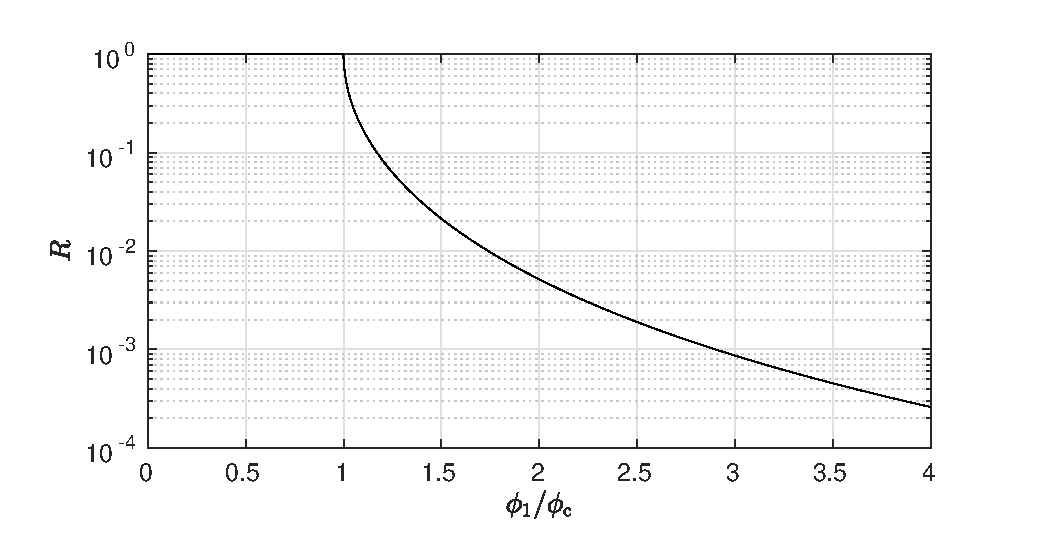
\includegraphics[width=.7\textwidth]{3d_R.eps}
\caption{The reflectivity as a function of $\phi_1/\phic$. Note the
  log scale on the $R$ axis.}
\label{fig:3d_R}
\end{figure}

One interesting thing to note here is that $R=1$ as soon as
$\phi_1\le\phic$, since then the square roots become imaginary and the
absolute values in the numerator and denominator then are equal. 
A plot of $R$ as a function of $\xi=\phi_1/\phic$, can be found in
\figref{fig:3d_R}. 




\section{Dispersion relation in conducting media}
Starting off from the Maxwell equation
\begin{equation}
\curl\vb*B = \mu\vb*J + \mu\epsilon\pdv{\vb*E}{t},
\end{equation}
we can introduce Ohm's law $\vb*J=\sigma\vb*E$ and take the curl of
both sides. We now have
\begin{equation}\label{eq:4_wave-eqn}
\curl[\curl\vb*B] = 
\curl\qty[\mu\sigma\vb*E + \mu\epsilon\pdv{\vb*E}{t}]
=-\mu\sigma\pdv{\vb*B}{t} - \mu\epsilon\pdv[2]{\vb*B}{t},
\end{equation}
where the last step was due to Faraday's law 
$\curl\vb*E = -\pdv{\vb*B}{t}$ and the fact that the partial
derivative commute $\curl\pdv{\vb*E}{t} = \pdv{\curl\vb*E}{t}$. 
Next we need to use the vector identity
\begin{equation}
\curl(\curl\vb*B) = \grad{}(\cancelto{0}{\div\vb*B}) - \laplacian\vb*B.
\end{equation}
The first term is canceled by the ``no monopoles Maxwell
equation''. All together we therefore have
\begin{equation}\label{eq:4_wave-eqn}
\laplacian\vb*B
-\mu\sigma\pdv{\vb*B}{t} - \mu\epsilon\pdv[2]{\vb*B}{t} =0
\end{equation}

We now have a (damped) wave equation for the $\vb*B$ field. Assuming
harmonic solutions
\begin{equation}
\vb*B(\vb*r, t) = B_0\ee^{\ii\vb*k\vdot\vb*r - \ii\omega t}\vu{n}
\end{equation}
we can get a dispersion relation by substituting this into
\eqref{eq:4_wave-eqn}. We then get
\begin{equation}
\qty[(\ii\vb*k)^2
-\mu\sigma(-\ii\omega) - \mu\epsilon(-\ii\omega)^2
]B_0\ee^{\ii\vb*k\vdot\vb*r - \ii\omega t}\vu{n} =0.
\end{equation}
Now, the things outside the brackets are not always 0, so instead what
is inside the brackets must be 0. I.e.
\begin{equation}
0=(\ii\vb*k)^2
-\mu\sigma(-\ii\omega) - \mu\epsilon(-\ii\omega)^2
\end{equation}
or when cleaned up
\begin{equation}\label{eq:4_disp}
\kt^2 = \ii\mu\sigma\omega +\mu\epsilon\omega^2,
\end{equation}
where $\kt^2 = \vb*k\vdot\vb*k$.
This is our dispersion relation for an Ohmic conductive media. 



Now, we want to prove that $\kt=k+\ii\kappa$ will satisfy
\eqref{eq:4_disp} with
\begin{equation}\label{eq:4_ktilde}
k=\omega\sqrt{\frac{\epsilon\mu}{2}}
\qty[\sqrt{1+\qty(\frac{\sigma}{\epsilon\omega})^2}+1]^{1/2}
\qcomma
\kappa=\omega\sqrt{\frac{\epsilon\mu}{2}}
\qty[\sqrt{1+\qty(\frac{\sigma}{\epsilon\omega})^2}-1]^{1/2}.
\end{equation}
The easiest way would be to just substitute \eqref{eq:4_ktilde} into
\eqref{eq:4_disp}, but I guess that would be a bit cheating. So
instead we substitute $\kt=k+\ii\kappa$ into \eqref{eq:4_disp}. We then
get
\begin{equation}
k^2-\kappa^2 + 2\ii k\kappa 
= \ii\mu\sigma\omega +\mu\epsilon\omega^2.
\end{equation}
We know that the real and imaginary parts both have to be equal, which
gives us two equations. From the imaginary part we get
\begin{equation}
\kappa=\frac{\mu\sigma\omega}{2k}.
\end{equation}
When we put this into the equation for the real part we get
\begin{equation}
k^2- \qty(\frac{\mu\sigma\omega}{2k})^2
= \mu\epsilon\omega^2.
\end{equation}
Multiplying both sides by $k^2$ and moving every thing to one side
yields 
\begin{equation}
k^4- \qty(\frac{\mu\sigma\omega}{2})^2
- k^2\mu\epsilon\omega^2 =0.
\end{equation}
This is a quadratic equation in the variable $k^2$, which has the
solutions
\begin{equation}\label{eq:4_k2}
\begin{aligned}
k^2 =& \frac{\mu\epsilon\omega^2}{2}
\pm\sqrt{
\qty(\frac{\mu\epsilon\omega^2}{2})^2 
+ \qty(\frac{\mu\sigma\omega}{2})^2   }\\
=& \frac{\mu\epsilon\omega^2}{2}
\qty[ 1 \pm\sqrt{
1+ \qty(\frac{\mu\sigma\omega}{\mu\epsilon\omega^2})^2
} ].
\end{aligned}
\end{equation}
For just the value $k$, we see that the square root is greater than 1,
so to keep $k$ real we must choose the ``+'' solution. We therefore
end up with
\begin{equation}
k = \omega\sqrt{\frac{\mu\epsilon}{2}}
\qty[ 1 +\sqrt{
1+ \qty(\frac{\sigma}{\epsilon\omega})^2
} ]^{1/2}.
\end{equation}
To get $\kappa$, we use 
\begin{equation}
k^2-\kappa^2 = \mu\epsilon\omega^2
\end{equation}
together with \eqref{eq:4_k2}. This gives
\begin{equation}
\begin{aligned}
\kappa^2 =& k^2-\mu\epsilon\omega^2\\
=&\frac{\mu\epsilon\omega^2}{2}
\qty[ 1 +\sqrt{
1+ \qty(\frac{\mu\sigma\omega}{\mu\epsilon\omega^2})^2
} ]
-\mu\epsilon\omega^2\\
=&\frac{\mu\epsilon\omega^2}{2}
\qty[ -1 +\sqrt{
1+ \qty(\frac{\mu\sigma\omega}{\mu\epsilon\omega^2})^2
} ].
\end{aligned}
\end{equation}
And the ``un-squared'' value is
\begin{equation}
\kappa = \omega\sqrt{\frac{\mu\epsilon}{2}}
\qty[ -1 +\sqrt{
1+ \qty(\frac{\sigma}{\epsilon\omega})^2
} ]^{1/2}.
\end{equation}
Both the expressions for $k$ and $\kappa$ are exactly the same as
\eqref{eq:4_ktilde}. We are thereby done.








\end{document}




%  LocalWords:  wavenumber wavevectors Mathematica
%  LocalWords:  reflectivity transmitivity
